% Gallery figure source
% Summary: Tree space versus network space on a fixed leaf set. The left panel shows the entire unrooted binary tree space for four leaves. The right panel shows why unconstrained phylogenetic network space is unbounded: reticulate structures can be added repeatedly while the observed leaves remain $A,B,C,D$.
\documentclass[tikz,border=6pt]{standalone}
% Shared color palette
\usepackage[T1]{fontenc}
\usepackage[utf8]{inputenc}
\usepackage{lmodern}
\usepackage{microtype}
\usepackage{amsmath,amssymb,mathtools}
\usepackage{xcolor}
\usepackage{tikz}
\usetikzlibrary{arrows.meta,positioning,calc,fit,backgrounds,decorations.pathreplacing,shapes.geometric,shadows.blur}

\definecolor{mainblue}{RGB}{42,85,132}
\definecolor{deepgreen}{RGB}{30,105,70}
\definecolor{burntorange}{RGB}{190,90,25}
\definecolor{softgray}{RGB}{245,246,248}
\definecolor{darkgray}{RGB}{70,70,70}
\definecolor{violet}{RGB}{110,70,150}

\newcommand{\given}{\,|\,}
\newcommand{\Ne}{N_{e}}
\newcommand{\ARG}{\mathrm{ARG}}
\newcommand{\MRCA}{\mathrm{MRCA}}
\newcommand{\GMRCA}{\mathrm{GMRCA}}

% Shared TikZ styles
\tikzset{
  tip/.style={circle,fill=black,inner sep=1.6pt},
  nodept/.style={circle,fill=black,inner sep=1.4pt},
  sampled/.style={rectangle,fill=black,inner sep=2.2pt},
  branch/.style={line width=0.8pt},
  retic/.style={circle,draw=burntorange,fill=burntorange!25,line width=0.8pt,inner sep=2.0pt},
  event/.style={circle,draw=mainblue,fill=mainblue!15,line width=0.8pt,inner sep=1.8pt},
  arr/.style={-{Latex[length=2.0mm]},line width=0.8pt},
  faint/.style={line width=0.7pt,draw=gray!55},
  parentedge/.style={-{Latex[length=2.0mm]},line width=0.9pt,draw=burntorange},
  treeedge/.style={-{Latex[length=2.0mm]},line width=0.9pt,draw=black},
  segment/.style={line width=4pt,line cap=round},
  dashedretic/.style={-{Latex[length=2.0mm]},line width=0.9pt,draw=burntorange,dashed}
}


\begin{document}
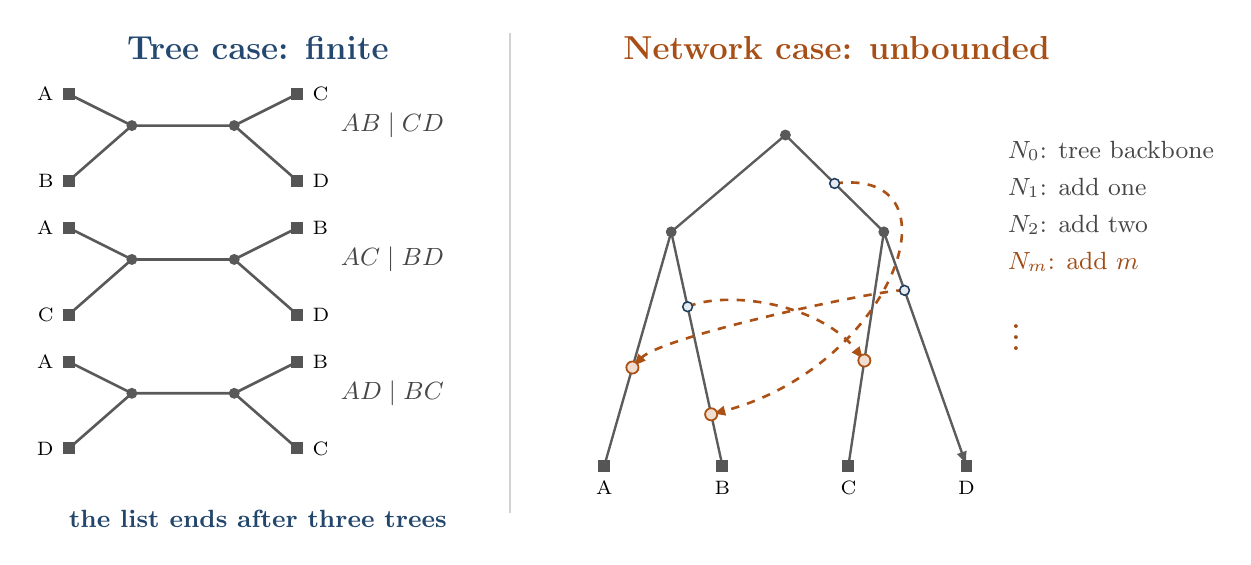
\begin{tikzpicture}[
  scale=1.0,
  paneltitle/.style={font=\bfseries\large},
  treeline/.style={line width=.95pt,draw=darkgray!90,line cap=round},
  netline/.style={-{Latex[length=1.8mm]},line width=.86pt,draw=darkgray!88,line cap=round},
  retline/.style={-{Latex[length=1.8mm]},line width=.95pt,dashed,draw=burntorange!90!black},
  intnode/.style={circle,fill=darkgray!90,inner sep=1.4pt},
  tipmark/.style={rectangle,fill=darkgray!92,inner sep=2.15pt},
  retnode/.style={circle,draw=burntorange!90!black,fill=burntorange!20,line width=.65pt,inner sep=1.55pt},
  sourcenode/.style={circle,draw=mainblue!70!black,fill=mainblue!12,line width=.55pt,inner sep=1.25pt},
  splitlabel/.style={font=\small\bfseries,text=darkgray},
  expl/.style={font=\small,align=center,text width=5.8cm,text=darkgray},
  eq/.style={font=\small,align=left,text=darkgray}
]

\begin{scope}
  \node[paneltitle,text=mainblue!85!black] at (2.85,6.15)
    {Tree case: finite};

  \begin{scope}[xshift=0.20cm,yshift=4.35cm]
    \coordinate (uL) at (1.05,0.82);
    \coordinate (uR) at (2.35,0.82);
    \coordinate (A) at (0.25,1.22);
    \coordinate (B) at (0.25,0.12);
    \coordinate (C) at (3.15,1.22);
    \coordinate (D) at (3.15,0.12);

    \draw[treeline] (uL)--(uR)
                    (uL)--(A)
                    (uL)--(B)
                    (uR)--(C)
                    (uR)--(D);

    \foreach \p in {uL,uR}{
      \node[intnode] at (\p) {};
    }

    \node[tipmark] at (A) {};
    \node[left=2pt,font=\scriptsize] at (A) {A};
    \node[tipmark] at (B) {};
    \node[left=2pt,font=\scriptsize] at (B) {B};
    \node[tipmark] at (C) {};
    \node[right=2pt,font=\scriptsize] at (C) {C};
    \node[tipmark] at (D) {};
    \node[right=2pt,font=\scriptsize] at (D) {D};

    \node[splitlabel,anchor=west] at (3.58,0.82) {$AB\mid CD$};
  \end{scope}

  \begin{scope}[xshift=0.20cm,yshift=2.65cm]
    \coordinate (uL) at (1.05,0.82);
    \coordinate (uR) at (2.35,0.82);
    \coordinate (A) at (0.25,1.22);
    \coordinate (C) at (0.25,0.12);
    \coordinate (B) at (3.15,1.22);
    \coordinate (D) at (3.15,0.12);

    \draw[treeline] (uL)--(uR)
                    (uL)--(A)
                    (uL)--(C)
                    (uR)--(B)
                    (uR)--(D);

    \foreach \p in {uL,uR}{
      \node[intnode] at (\p) {};
    }

    \node[tipmark] at (A) {};
    \node[left=2pt,font=\scriptsize] at (A) {A};
    \node[tipmark] at (C) {};
    \node[left=2pt,font=\scriptsize] at (C) {C};
    \node[tipmark] at (B) {};
    \node[right=2pt,font=\scriptsize] at (B) {B};
    \node[tipmark] at (D) {};
    \node[right=2pt,font=\scriptsize] at (D) {D};

    \node[splitlabel,anchor=west] at (3.58,0.82) {$AC\mid BD$};
  \end{scope}

  \begin{scope}[xshift=0.20cm,yshift=0.95cm]
    \coordinate (uL) at (1.05,0.82);
    \coordinate (uR) at (2.35,0.82);
    \coordinate (A) at (0.25,1.22);
    \coordinate (D) at (0.25,0.12);
    \coordinate (B) at (3.15,1.22);
    \coordinate (C) at (3.15,0.12);

    \draw[treeline] (uL)--(uR)
                    (uL)--(A)
                    (uL)--(D)
                    (uR)--(B)
                    (uR)--(C);

    \foreach \p in {uL,uR}{
      \node[intnode] at (\p) {};
    }

    \node[tipmark] at (A) {};
    \node[left=2pt,font=\scriptsize] at (A) {A};
    \node[tipmark] at (D) {};
    \node[left=2pt,font=\scriptsize] at (D) {D};
    \node[tipmark] at (B) {};
    \node[right=2pt,font=\scriptsize] at (B) {B};
    \node[tipmark] at (C) {};
    \node[right=2pt,font=\scriptsize] at (C) {C};

    \node[splitlabel,anchor=west] at (3.58,0.82) {$AD\mid BC$};
  \end{scope}

  \node[font=\small\bfseries,text=mainblue!82!black] at (2.85,0.18)
    {the list ends after three trees};
\end{scope}

\draw[gray!35,line width=.6pt] (6.05,0.25)--(6.05,6.35);

\begin{scope}[xshift=6.70cm]
  \node[paneltitle,text=burntorange!88!black] at (3.50,6.15)
    {Network case: unbounded};

  \coordinate (r)  at (2.85,5.05);
  \coordinate (nL) at (1.40,3.82);
  \coordinate (nR) at (4.10,3.82);
  \coordinate (A)  at (0.55,0.85);
  \coordinate (B)  at (2.05,0.85);
  \coordinate (C)  at (3.65,0.85);
  \coordinate (D)  at (5.15,0.85);

  \coordinate (sOne)   at ($(nL)!0.32!(B)$);
  \coordinate (hOne)   at ($(nR)!0.55!(C)$);
  \coordinate (sTwo)   at ($(nR)!0.25!(D)$);
  \coordinate (hTwo)   at ($(nL)!0.58!(A)$);
  \coordinate (sThree) at ($(r)!0.50!(nR)$);
  \coordinate (hThree) at ($(nL)!0.78!(B)$);

  \draw[netline] (r)--(nL)
                 (r)--(nR)
                 (nL)--(A)
                 (nL)--(B)
                 (nR)--(C)
                 (nR)--(D);

  \draw[retline] (sOne) .. controls (2.10,3.08) and (3.28,2.92) .. (hOne);
  \draw[retline] (sTwo) .. controls (4.10,3.10) and (1.28,2.50) .. (hTwo);
  \draw[retline] (sThree) .. controls (5.15,4.65) and (4.20,2.10) .. (hThree);

  \node[sourcenode] at (sOne) {};
  \node[retnode] at (hOne) {};
  \node[sourcenode] at (sTwo) {};
  \node[retnode] at (hTwo) {};
  \node[sourcenode] at (sThree) {};
  \node[retnode] at (hThree) {};

  \foreach \p in {r,nL,nR}{
    \node[intnode] at (\p) {};
  }

  \foreach \p/\lab in {A/A,B/B,C/C,D/D}{
    \node[tipmark] at (\p) {};
    \node[below=2pt,font=\scriptsize] at (\p) {\lab};
  }

  \node[eq,anchor=west] at (5.55,4.85) {$N_0$: tree backbone};
  \node[eq,anchor=west] at (5.55,4.38) {$N_1$: add one};
  \node[eq,anchor=west] at (5.55,3.91) {$N_2$: add two};
  \node[eq,anchor=west,text=burntorange!85!black] at (5.55,3.44) {$N_m$: add $m$};
  \node[font=\Large,text=burntorange!85!black] at (5.78,2.58) {$\vdots$};
\end{scope}

\end{tikzpicture}
\end{document}
